\documentclass[border=3mm]{standalone}
\usepackage[T1]{fontenc}
\usepackage[utf8]{inputenc}
\usepackage{graphicx}
\usepackage{tikz}
\usetikzlibrary{arrows.meta,calc,positioning,shapes.geometric}
\setlength{\parindent}{0pt}

\definecolor{darktext}{RGB}{34,40,49}
\definecolor{panelborder}{RGB}{120,126,140}
\definecolor{lightgrayfill}{RGB}{243,244,246}
\definecolor{graybar}{RGB}{168,176,188}
\definecolor{bestred}{RGB}{217,83,79}
\definecolor{secretaryblue}{RGB}{39,110,241}
\definecolor{secretaryfill}{RGB}{220,233,255}
\definecolor{thresholdorange}{RGB}{233,140,53}
\definecolor{ertfill}{RGB}{197,244,214}
\definecolor{ertgreen}{RGB}{47,158,79}

\tikzset{
panel/.style={draw=panelborder, rounded corners=4pt, line width=0.5pt},
methodarrow/.style={-{Latex[length=2mm]}, line width=0.9pt, draw=panelborder},
ptitle/.style={font=\bfseries\small, text=darktext},
psubtitle/.style={font=\scriptsize, text=darktext, align=center},
labelsmall/.style={font=\scriptsize, text=darktext, align=center},
takeaway/.style={draw=panelborder, rounded corners=4pt, fill=lightgrayfill, inner sep=7pt, font=\footnotesize, text=darktext},
explabel/.style={font=\scriptsize\bfseries, text=secretaryblue},
selabel/.style={font=\scriptsize\bfseries, text=darktext},
beststar/.style={star, star points=5, fill=bestred, draw=bestred, minimum size=5mm},
beststargreen/.style={star, star points=5, fill=ertgreen, draw=ertgreen, minimum size=5mm}
}

\begin{document}
\fbox{%
\begin{minipage}[t][10.9cm][t]{17.15cm}
\vspace*{0.18cm}
{\small\bfseries Secretary-style split search for decision trees\par}
{\footnotesize Mathias Valla\par}
\vspace{0.32cm}
\centering
\resizebox{15.10cm}{!}{%
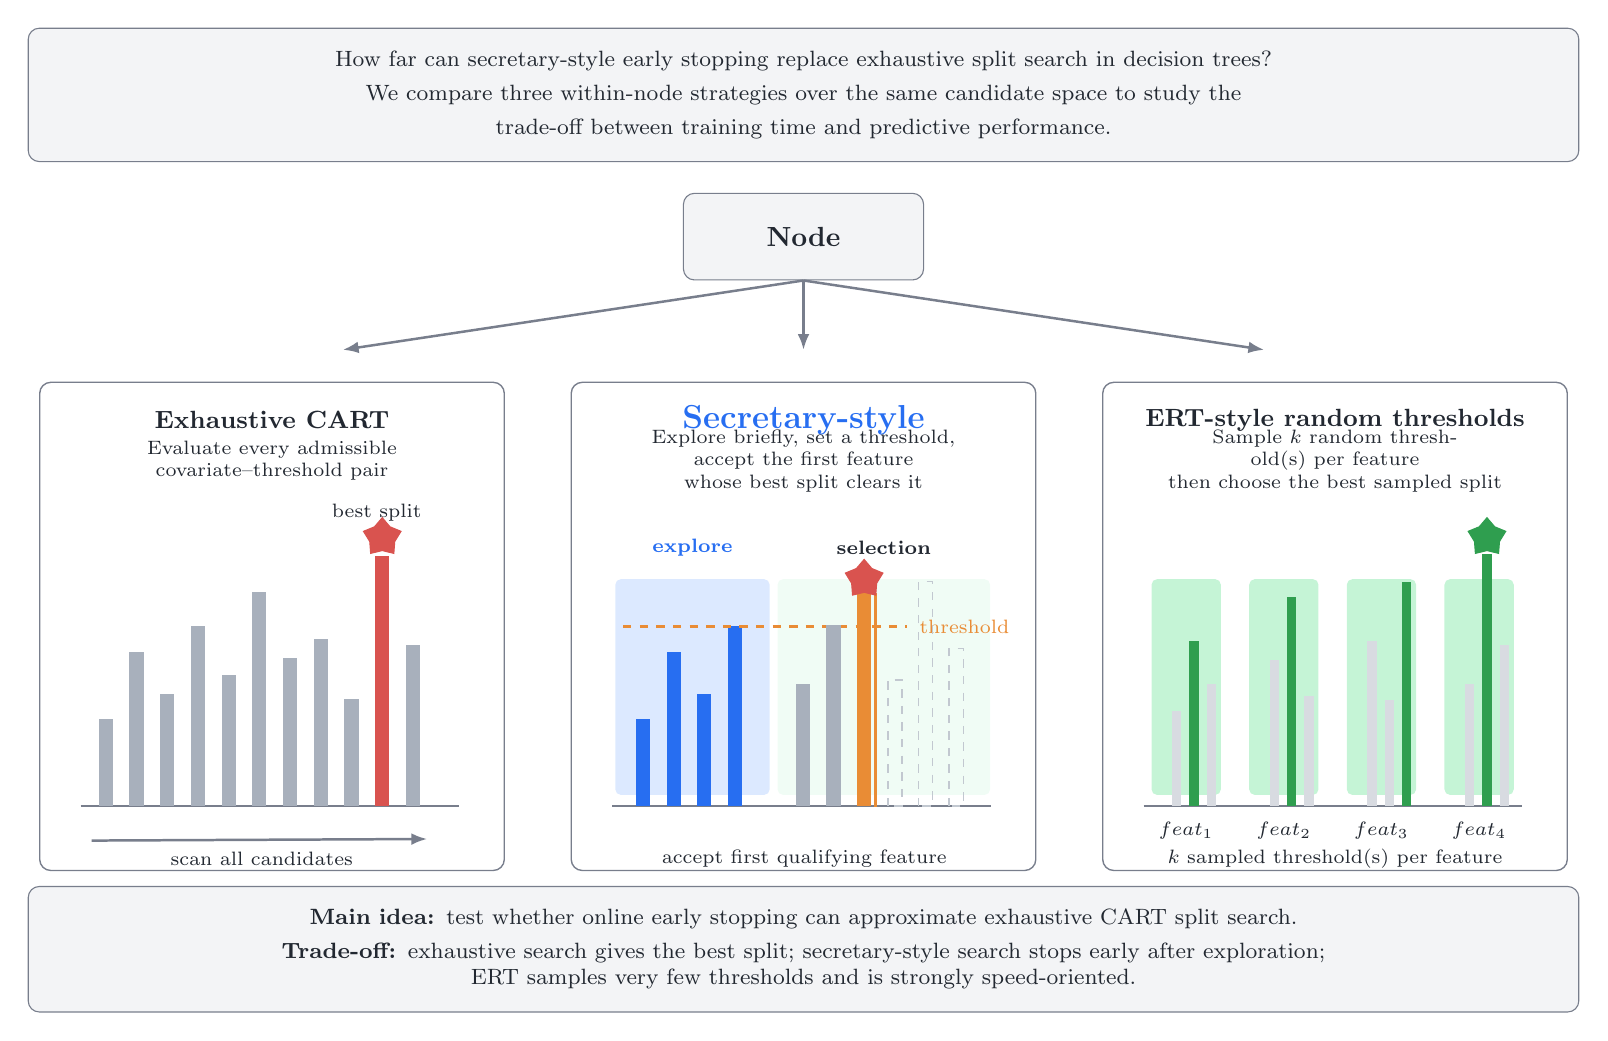
\begin{tikzpicture}[x=1cm,y=1cm]

\node[takeaway, text width=19.2cm, align=center] at (10.0,8.10)
{
\begin{tabular}{c}
How far can secretary-style early stopping replace exhaustive split search in decision trees?\\[1mm]
We compare three within-node strategies over the same candidate space to study the\\[1mm]
trade-off between training time and predictive performance.
\end{tabular}
};

\node[
  draw=panelborder,
  rounded corners=4pt,
  minimum width=3.05cm,
  minimum height=1.10cm,
  fill=lightgrayfill,
  font=\bfseries,
  text=darktext
] (nodebox) at (10.0,6.30) {Node};

\draw[methodarrow] (nodebox.south) -- ++(-5.85,-0.88);
\draw[methodarrow] (nodebox.south) -- ++(0,-0.88);
\draw[methodarrow] (nodebox.south) -- ++(5.85,-0.88);

\def\Ytop{4.45}
\def\PanelH{6.20}
\def\PanelW{5.90}

\coordinate (P1) at (0.30,\Ytop-\PanelH);
\coordinate (P2) at (7.05,\Ytop-\PanelH);
\coordinate (P3) at (13.80,\Ytop-\PanelH);

\draw[panel] (P1) rectangle ++(\PanelW,\PanelH);
\node[ptitle] at ($(P1)+(2.95,5.72)$) {Exhaustive CART};
\node[psubtitle, text width=4.80cm] at ($(P1)+(2.95,5.20)$)
{Evaluate every admissible\\covariate--threshold pair};

\draw[line width=0.5pt, draw=panelborder] ($(P1)+(0.52,0.82)$) -- ($(P1)+(5.33,0.82)$);

\foreach \x/\h in {
0.75/1.10, 1.14/1.95, 1.53/1.42, 1.92/2.28, 2.31/1.66,
2.70/2.72, 3.09/1.88, 3.48/2.12, 3.87/1.36, 4.26/3.18, 4.65/2.04} {
  \fill[graybar] ($(P1)+(\x,0.82)$) rectangle ++(0.18,\h);
}

\fill[bestred] ($(P1)+(4.26,0.82)$) rectangle ++(0.18,3.18);
\node[beststar] at ($(P1)+(4.35,4.23)$) {};
\node[labelsmall] at ($(P1)+(4.28,4.55)$) {best split};

\draw[methodarrow] ($(P1)+(0.66,0.38)$) -- ($(P1)+(4.92,0.4)$);
\node[labelsmall] at ($(P1)+(2.82,0.15)$) {scan all candidates};

\draw[panel] (P2) rectangle ++(\PanelW,\PanelH);
\node[ptitle, text=secretaryblue] at ($(P2)+(2.95,5.72)$) {\large Secretary-style};
\node[psubtitle, text width=4.95cm] at ($(P2)+(2.95,5.20)$)
{Explore briefly, set a threshold,\\accept the first feature whose best split clears it};

\fill[secretaryfill, rounded corners=2pt] ($(P2)+(0.56,0.96)$) rectangle ($(P2)+(2.52,3.70)$);
\fill[ertfill!25, rounded corners=2pt] ($(P2)+(2.62,0.96)$) rectangle ($(P2)+(5.32,3.70)$);

\node[explabel] at ($(P2)+(1.54,4.10)$) {explore};
\node[selabel] at ($(P2)+(3.97,4.10)$) {selection};

\draw[line width=0.5pt, draw=panelborder] ($(P2)+(0.52,0.82)$) -- ($(P2)+(5.33,0.82)$);

\foreach \x/\h in {
0.82/1.10, 1.21/1.95, 1.60/1.42, 1.99/2.28} {
  \fill[secretaryblue] ($(P2)+(\x,0.82)$) rectangle ++(0.18,\h);
}

\draw[dashed, line width=0.9pt, draw=thresholdorange] ($(P2)+(0.66,3.10)$) -- ($(P2)+(4.26,3.10)$);
\node[labelsmall, anchor=west, text=thresholdorange] at ($(P2)+(4.30,3.10)$) {threshold};

\fill[graybar] ($(P2)+(2.85,0.82)$) rectangle ++(0.18,1.55);
\fill[graybar] ($(P2)+(3.24,0.82)$) rectangle ++(0.18,2.30);
\fill[thresholdorange] ($(P2)+(3.63,0.82)$) rectangle ++(0.18,2.7);

\foreach \x/\h in {4.02/1.60, 4.41/2.85, 4.80/2.00} {
  \draw[draw=graybar!70, dashed, line width=0.6pt] ($(P2)+(\x,0.82)$) rectangle ++(0.18,\h);
}

\draw[line width=1.0pt, draw=thresholdorange] ($(P2)+(3.86,0.81)$) -- ($(P2)+(3.86,3.52)$);
\node[beststar] at ($(P2)+(3.72,3.7)$) {};

\node[labelsmall] at ($(P2)+(2.96,0.15)$) {accept first qualifying feature};

\draw[panel] (P3) rectangle ++(\PanelW,\PanelH);
\node[ptitle] at ($(P3)+(2.95,5.72)$) {ERT-style random thresholds};
\node[psubtitle, text width=5.00cm] at ($(P3)+(2.95,5.20)$)
{Sample $k$ random threshold(s) per feature\\then choose the best sampled split};

\foreach \xa in {0.62, 1.86, 3.10, 4.34} {
  \fill[ertfill, rounded corners=2pt] ($(P3)+(\xa,0.96)$) rectangle ++(0.88,2.74);
}

\node[labelsmall] at ($(P3)+(1.06,0.5)$) {$feat_1$};
\node[labelsmall] at ($(P3)+(2.30,0.5)$) {$feat_2$};
\node[labelsmall] at ($(P3)+(3.54,0.5)$) {$feat_3$};
\node[labelsmall] at ($(P3)+(4.78,0.5)$) {$feat_4$};

\draw[line width=0.5pt, draw=panelborder] ($(P3)+(0.52,0.82)$) -- ($(P3)+(5.33,0.82)$);

\foreach \x/\h in {
0.88/1.20, 1.10/2.10, 1.32/1.55,
2.12/1.85, 2.34/2.65, 2.56/1.40,
3.36/2.10, 3.58/1.35, 3.80/2.85,
4.60/1.55, 4.82/3.20, 5.04/2.05} {
  \fill[graybar!45] ($(P3)+(\x,0.82)$) rectangle ++(0.12,\h);
}

\fill[ertgreen] ($(P3)+(1.10,0.82)$) rectangle ++(0.12,2.10);
\fill[ertgreen] ($(P3)+(2.34,0.82)$) rectangle ++(0.12,2.65);
\fill[ertgreen] ($(P3)+(3.80,0.82)$) rectangle ++(0.12,2.85);
\fill[ertgreen] ($(P3)+(4.82,0.82)$) rectangle ++(0.12,3.2);

\node[beststargreen] at ($(P3)+(4.88,4.23)$) {};
\node[labelsmall] at ($(P3)+(2.95,0.15)$) {$k$ sampled threshold(s) per feature};

\node[takeaway, text width=19.2cm, align=center] at (10.0,-2.75)
{
\begin{tabular}{c}
\textbf{Main idea:} test whether online early stopping can approximate exhaustive CART split search.\\[1mm]
\textbf{Trade-off:} exhaustive search gives the best split; secretary-style search stops early after exploration;\\
ERT samples very few thresholds and is strongly speed-oriented.
\end{tabular}
};

\end{tikzpicture}}
\end{minipage}}
\end{document}
